\setcounter{section}{41}
\setcounter{ex}{0}
\section{Cực trị của số phức}
\subsection{Kiến thức cần nhớ}
\begin{khung}
	\subsubsection{Môđun của số phức}
	Số phức $ z=a+bi $ được biểu diễn bởi điểm $ M(x;y) $ trên mặt phẳng $ Oxy $. Độ dài véc-tơ $ \vv{OM} $ được gọi là môđun của số phức $ z $.\\
	Kí hiệu $ |z|=\sqrt{a^2+b^2} $.\\
	Tính chất:
	\begin{itemize}
		\item $ |z|=\sqrt{a^2+b^2}=\sqrt{z\cdot \overline{z}}=|\vv{OM}| $.
		\item $ |z|\ge 0,\forall z\in\mathbb{C} $, $ |z|=0\Leftrightarrow z=0 $.
		\item $ |z\cdot z'|=|z|\cdot |z'| $, $ \left|\dfrac{z}{z'}\right|=\dfrac{|z|}{|z'|}, z'\ne 0 $.
		\item $ \left||z|-|z'|\right|\le |z\pm z'|\le |z|+|z'| $.
		\item $ |kz|=|k|.\cdot|z|, k\in\mathbb{R} $.
		\item $ |z|^2=z\cdot \overline{z}=a^2+b^2 $.
	\end{itemize}
	Một số bất đẳng thức:
	\begin{itemize}
		\item $ |z_1+z_2|\le |z_1|+|z_2| $ dấu bằng xảy ra khi và chỉ khi $ z_1=kz_2 $ $ (k\ge 0) $.
		\item $ |z_1-z_2|\le |z_1|+|z_2| $ dấu bằng xảy ra khi và chỉ khi $ z_1=kz_2 $ $ (k\le 0) $.
		\item $ |z_1+z_2|\ge \left||z_1|-|z_2|\right| $ dấu bằng xảy ra khi và chỉ khi $ z_1=kz_2 $ $ (k\le 0) $.
		\item $ |z_1-z_2|\ge \left||z_1|-|z_2|\right| $ dấu bằng xảy ra khi và chỉ khi $ z_1=kz_2 $ $ (k\ge 0) $.
	\end{itemize}
	
\end{khung}
\subsection{Bài tập mẫu}
\begin{khung}
	\begin{vd}%[2D4K5-2]%[Huỳnh Thanh Chí]
		[Đề minh họa BGD 2022-2023]
		Xét các số phức $ z $ thỏa mãn $ |z^2-3-4i|=2|z| $. Gọi $ M $ và $ m $ lần lượt là giá trị lớn nhất và giá trị nhỏ nhất của $ |z| $. Giá trị của $ M^2+m^2 $ bằng
		\choice
		{$ 28 $}
		{$ 18+4\sqrt{6} $}
		{\True $ 14 $}
		{$ 11+4\sqrt{6} $}
		\loigiai{Ta có
			\begin{eqnarray*}
				&& 2|z|=|z^2-3-4i|\ge ||z|-|3+4i||\\
				&\Leftrightarrow& 2|z| \ge ||z|^2-5| \Leftrightarrow 2|z|\ge |z|^2-5\ge -2|z|\\
				&\Leftrightarrow& \heva{& |z|^2-2|z|-5\le 0\\ & |z|^2+2|z|-5\ge 0} \Leftrightarrow \heva{& |z|\le 1+\sqrt{6}\\ & |z| \ge -1+\sqrt{6}}\\
				&\Leftrightarrow& \heva{& M=1+\sqrt{6}\\ & m=-1+\sqrt{6}} \Rightarrow M^2+m^2=14.
		\end{eqnarray*}}
	\end{vd}
\end{khung}

\subsection{Bài tập tương tự và phát triển}	
\Opensolutionfile{ans}[ans/ANS-DANG-42]
	\begin{ex}%[2D4K5-2]%[Huỳnh Thanh Chí]
	Xét tập hợp $S$ các số phức $x+yi\left( x,y\in \mathbb{R} \right)$ thỏa mãn điều kiện $\left| 3z-\overline{z} \right|=\left| \left( 1+i \right)\left( 2+2i \right) \right|$. Biểu thức $Q=\left| z-\overline{z} \right|\left( 2-x \right)$ đạt giá trị lớn nhất là $M$ và đạt được tại $z_0=x_0+y_0i$ (khi $z$ thay đổi trong tập $S$). Tính giá trị của $T=M\cdot x_0\cdot y_0^2$.
	\choice
	{\True $T=-\dfrac{9\sqrt{3}}{4}$}
	{ $T=\dfrac{9\sqrt{3}}{4}$}
	{ $T=\dfrac{9\sqrt{3}}{2}$}
	{ $T=-\dfrac{9\sqrt{3}}{2}$}
	\loigiai{
		Ta có $\left| 2x+4yi \right|=4\Leftrightarrow {x^2}+4y^2=4\Rightarrow \heva{
			& -2\le x\le 2 \\
			& 4y^2=4-x^2. \\
		}$\\
		$\begin{aligned}
			& Q=\left| z-\overline{z} \right|\left( 2-x \right) \\
			& \Rightarrow {Q^2}={{\left( 2-x \right)}^2}{{\left| 4yi \right|}^2}={{\left( 2-x \right)}^2}\left( 4-x^2 \right)=\dfrac{1}{3}{{\left( 2-x \right)}^3}\left( 6+3x \right)\overset{AM-GM}{\mathop{\le }}\,\dfrac{1}{3}{{\left( \dfrac{6-3x+6+3x}{4} \right)}^4}=27 \\
		\end{aligned}$\\
		$\Rightarrow M=\dfrac{9}{\sqrt{3}}$ đạt được khi $\heva{
			& 2-x_0=6+3x_0 \\
			& 4y_0^2=4-x_0^2 \\
		}\Rightarrow \heva{
			& {x_0}=-1 \\
			& {y_0}^2=\dfrac{3}{4}. \\
		}$\\
		Suy ra $T=\dfrac{9}{\sqrt{3}}\cdot\left( -1 \right)\cdot\dfrac{3}{4}=-\dfrac{9\sqrt{3}}{4}$.}
\end{ex}
\begin{ex}%[2D4K5-2]%[Huỳnh Thanh Chí]
	Cho số phức z thỏa mãn $|z+1+2i|=2$. Gọi $M, m$ lần lượt là giá trị lớn nhất, giá trị nhỏ nhất của $|z^2+\left( 2+2i \right)z-1+2i|$. Giá trị của biểu thức $T=M^2+m^2$ bằng
	\choice
	{ $103$}
	{ $101$}
	{ $104$}
	{\True $102$}
	\loigiai{
		Đặt $A=|z^2+\left( 2+2i \right)z-1+2i|=|\left( z+i \right)\left( z+2+i \right)|$.\\
		Đặt $w =z+i$, $w =a+bi$, điểm $M(a;b)$ biểu diễn $w $.\\
		Theo đề bài $|z+1+2i|=2\Leftrightarrow |w +1+i|=2\Leftrightarrow {{\left( a+1 \right)}^2}+{{\left( b+1 \right)}^2}=4\Leftrightarrow {a^2}+b^2=2-2a-2b$.\\
		Ta có 
		\allowdisplaybreaks
		\begin{eqnarray*}
			A &=& |w |\cdot|w +2|=\sqrt{a^2+b^2}\cdot\sqrt{\left( a+2 \right)^2+b^2}=\sqrt{\left( 2-2a-2b \right)\left( 6+2a-2b \right)} \\
			A &=& 2\sqrt{\left( 1-(a+b) \right)\left( 3+\left(a-b \right) \right)}=2\sqrt{3-2a-4b-a^2+b^2}=2\sqrt{{{\left( b-2 \right)}^2}-{{\left( a+1 \right)}^2}} \\
			A &=& 2\sqrt{\left( b-2 \right)^2+\left( b+1 \right)^2-4}=2\sqrt{2b^2-2b+1}=2\sqrt{f\left( b \right)}.
		\end{eqnarray*}
		Với $f\left( b \right)=2b^2-2b+1$, mà $-3\le b\le 1$ do ${{\left( b+1 \right)}^2}\le 4$.\\
		Ta có $ f'\left( b \right)=4b-2,\,f'\left( b \right)=0\Leftrightarrow b=\dfrac{1}{2}\in \left[ -3;1 \right] $.\\ 
		$f\left( -3 \right)=25,\,f\left( 1 \right)=1,\,f\left( \dfrac{1}{2} \right)=\dfrac{1}{2}.$\\
		Vậy $M=2\sqrt{25}=10;\,m=2\cdot\sqrt{\dfrac{1}{2}}=\sqrt{2}$ do đó $T=M^2+m^2=102$.}
\end{ex}
\begin{ex}%[2D4K5-2]%[Huỳnh Thanh Chí]
	Giả sử $z_1,z_2$ là hai nghiệm phức của phương trình $\left| \left( 2+i \right)\left| z \right|z-\left( 1-2i \right)z \right|=\left| 1+3i \right|$ và $\left| {z_1}-z_2 \right|=1$. Tính $M=\left| 2z_1+3z_2 \right|$.
	\choice
	{ $M=25$}
	{ $M=5$}
	{\True $M=\sqrt{19}$}
	{ $M=19$}
	\loigiai{
		Từ giả thiết, ta có $\left| \left( 2\left| z \right|-1 \right)+\left( \left| z \right|+2 \right)i \right|\cdot\left| z \right|=\sqrt{10}\Leftrightarrow \left[ \left( 2\left| z \right|-1 \right)^2+\left( \left| z \right|+2 \right)^2 \right]\cdot \left| z \right|^2=10$.\\
		$\Leftrightarrow 5{{\left| z \right|}^4}+5{{\left| z \right|}^2}-10=0\Leftrightarrow \left| z \right|=1$ (vì $\left| z \right|\ge 0$).\\
		Gọi $z_1=x_1+y_1i$ và $z_2=x_2+y_2i$. Ta có $\left| {z_1} \right|=\left| {z_2} \right|=1$ nên $x_1^2+y_1^2=x_2^2+y_2^2=1$.\\
		Mặt khác, $\left| {z_1}-z_2 \right|=1$ nên ${{\left( {x_1}-x_2 \right)}^2}+{{\left( {y_1}-y_2 \right)}^2}=1$. Suy ra $x_1{x_2}+y_1{y_2}=\dfrac{1}{2}$.\\
		Khi đó 
		\begin{eqnarray*}
			M &=& \left| 2z_1+3z_2 \right|=\sqrt{{{\left( 2x_1+3x_2 \right)}^2}+{{\left( 2y_1+3y_2 \right)}^2}} \\
			&=& \sqrt{4\left( x_1^2+y_1^2 \right)+9\left( x_2^2+y_2^2 \right)+12\left( {x_1}{x_2}+y_1{y_2} \right)}\\
			&=& \sqrt{4\cdot 1+9\cdot 1+12\cdot\dfrac{1}{2}}\\
			&=& \sqrt{19}.
		\end{eqnarray*}
		Vậy $M=\sqrt{19}$.}
\end{ex}
\begin{ex}%[2D4K5-2]%[Huỳnh Thanh Chí]
	Biết rằng $z$ là số phức có môđun nhỏ nhất thỏa mãn $\left( z-1 \right)\left( \overline{z}+2i \right)$ là số thực. Số phức $z$ là
	\choice
	{ $2i$}
	{\True $z=\dfrac{4}{5}+\dfrac{2}{5}i$}
	{ $z=1+\dfrac{1}{2}i$}
	{ $z=\dfrac{3}{5}+\dfrac{4}{5}i$}
	\loigiai{
		Gọi $z=x+iy$, với $x,y\in \mathbb{R}$. Khi đó $\left( z-1 \right)\left( \overline{z}+2i \right)=x\left( x-1 \right)+y(y-2)+\left( 2x+y-2 \right)i$.\\
		Từ giả thiết suy ra $2x+y-2=0$ hay $2x+y=2$.\\
		Ta có $4={{\left( 2x+y \right)}^2}\le 5\left( {x^2}+y^2 \right)\Leftrightarrow {x^2}+y^2\ge \dfrac{4}{5}\Leftrightarrow \sqrt{x^2+y^2}\ge \dfrac{2}{\sqrt{5}}$.\\
		Tức là $\left| z \right|=\sqrt{x^2+y^2}\ge \dfrac{2}{\sqrt{5}}$.\\
		Do đó $\min\left| z \right|=\dfrac{2}{\sqrt{5}}$ khi $\dfrac{x}{2}=\dfrac{y}{1}\Leftrightarrow x=2y$.\\
		Suy ra $x=\dfrac{4}{5};y=\dfrac{2}{5}$.\\
		Vậy $z=\dfrac{4}{5}+\dfrac{2}{5}i$.}
\end{ex}

\begin{ex}%[2D4K5-1]%[Huỳnh Thanh Chí]
	Cho số phức $z$ thỏa mãn $\left| z-1-2i \right|=\left| z-2+i \right|$. Đặt $w=z+2-3i$ tìm giá trị nhỏ nhất của $\left| w \right|$.
	\choice
	{ $\dfrac{\sqrt{30}}{2}$}
	{\True $\dfrac{11}{\sqrt{10}}$}
	{ $\dfrac{2\sqrt{15}}{5}$}
	{ $\dfrac{\sqrt{10}}{3}$}
	\loigiai{
		Đặt $w=x+yi$ với $\left( x,y\in \mathbb{R} \right)$\\
		Vì: $w=z+2-3i\Leftrightarrow z=w-2+3i$\\
		Do đó: $\left| z-1-2i \right|=\left| z-2+i \right|\Leftrightarrow \left| w-3+i \right|=\left| w-4+4i \right|$\\
		$\Leftrightarrow {{\left( x-3 \right)}^2}+{{\left( y+1 \right)}^2}={{\left( x-4 \right)}^2}+{{\left( y+4 \right)}^2}\Leftrightarrow \grave{\ }x-3y-11=0$.\\
		Tập hợp số phức $w$ là đường thẳng $x-3y-11=0$.\\
		Vây $\left| w \right|$ nhỏ nhất khi tọa độ của $w$ là hình chiếu của $O\left( 0;0 \right)$ trên đường thẳng $x-3y-11=0$.\\
		Do đó $w=\dfrac{11}{10}-\dfrac{33}{10}i$ nên $\left| w \right|=\dfrac{11}{\sqrt{10}}$.}
\end{ex}
\begin{ex}%[2D4K5-1]%[Huỳnh Thanh Chí]
	Nếu $z$ là số phức thỏa $\left| \overline{z} \right|=\left| z+2i \right|$ thì giá trị nhỏ nhất của $\left| z-i \right|+\left| z-4 \right|$ là
	\choice
	{\True $5$}
	{ $\sqrt{3}$}
	{ $4$}
	{ $2$}
	\loigiai{
		Đặt $z=x+yi$ với $x$, $y\in \mathbb{R}$ theo giả thiết $\left| {\overline{z}} \right|=\left| z+2i \right|\Leftrightarrow y=-1$.\\
		Vậy tập hợp các điểm biểu diễn số phức $z$ là đường thẳng $\left( d \right)\colon y=-1$.\\
		Gọi $A\left( 0;1 \right)$, $B\left( 4;0 \right)$ suy ra $\left| z-i \right|+\left| z-4 \right|=P$ là tổng khoảng cách từ điểm $M\left( x;-1 \right)$ đến hai điểm $A$, $B$.\\
		Thấy ngay $A\left( 0;1 \right)$ và $B\left( 4;0 \right)$ nằm cùng phía với $\left( d \right)$. Lấy điểm đối xứng với $A\left( 0;1 \right)$ qua đường thẳng $\left( d \right)$ ta được điểm $A'\left( 0;-3 \right)$.\\
		Do đó khoảng cách ngắn nhất là ${A}'B=\sqrt{3^2+4^2}=5$.}
\end{ex}
\begin{ex}%[2D4K5-1]%[Huỳnh Thanh Chí]
	Cho số phức $z$ và số phức $u=\left( z-i \right)\left( \overline{z}+i \right)+2z-3i$ thỏa mãn $\left| u+1 \right|-\left| \overline{u}-i \right|=0$. Giá trị lớn nhất của biểu thức $T=\left| z-2+3i \right|$ bằng
	\choice
	{ $3+\sqrt{17}$}
	{ $\sqrt{34}-1$}
	{\True $1+\sqrt{34}$}
	{ $2+\sqrt{13}$}
	\loigiai{
		Gọi $u=x+yi$ với $x,y\in \mathbb{R} $.\\
		Suy ra hệ thức $\left| u+1 \right|-\left| \overline{u}-i \right|=0\Leftrightarrow \left| x+yi+1 \right|=\left| x-yi-i \right| $\\
		$ \Leftrightarrow \sqrt{{{\left( x+1 \right)}^2}+y^2}=\sqrt{x^2+{{\left( y+1 \right)}^2}}\Leftrightarrow x=y\Rightarrow $ số phức $u$ có phần thực bằng phần ảo.\\
		Gọi $z=a+bi$ với $a,b\in \mathbb{R} $
		\allowdisplaybreaks
		\begin{eqnarray*}
			\Rightarrow u &=& \left( z-i \right)\left( \overline{z}+i \right)+2z-3i \\
			&=& \left| z \right|^2+i\left( z-\overline{z} \right)+1+2z-3i\\
			&=& a^2+b^2+i\left( 2bi \right)+1+2\left( a+bi \right)-3i\\
			&=& \left( {a^2}+b^2+2a-2b+1 \right)+\left( 2b-3 \right)i.
		\end{eqnarray*}
		Suy ra: $\left( {a^2}+b^2+2a-2b+1 \right)=\left( 2b-3 \right)\Leftrightarrow {{\left( a+1 \right)}^2}+{{\left( b-2 \right)}^2}=1$\\
		Suy ra quỹ tích điểm biểu diễn số phức $z$ là đường tròn $\left( C \right)$ có tâm $I\left( -1;2 \right)$ và bán kính $R=1$.\\
		Biểu thức $T=\left| z-\left( 2-3i \right) \right|=MA$, với điểm $M$ biểu diễn số phức $z$ và nằm trên đường tròn $\left( C \right)$; điểm $A\left( 2;-3 \right)$.\\
		Suy ra $T=MA\le MI+IA=R+IA=1+\sqrt{34}$.}
\end{ex}
\begin{ex}%[2D4K5-1]%[Huỳnh Thanh Chí]
	Nếu $z$ là số phức thỏa mãn $\left| \overline{z} \right|=\left| z+2i \right|$ thì giá trị nhỏ nhất của $\left| z-i \right|+\left| z-4 \right|$ là
	\choice
	{ $4$}
	{ $2$}
	{ $\sqrt{3}$}
	{\True $5$}
	\loigiai{
		Đặt $z=x+yi$ biểu diễn điểm $M\left( x;y \right)$.\\
		$\left| \overline{z} \right|=\left| z+2i \right|\Leftrightarrow y=-1$.\\
		$\left| z-i \right|+\left| z-4 \right|$ nhỏ nhất $\Leftrightarrow MA+MB$ nhỏ nhất, với $A\left( 0;1 \right)$, $B\left( 4;0 \right)$.\\
		Gọi ${B}'$ đối xứng với $B$ qua đường thẳng $y=-1$ suy ra ${B}'\left( 4;-2 \right)$.\\
		Do đó, $MA+MB=MA+M{B}'\ge A{B}'=5$.}
\end{ex}
\begin{ex}%[2D4K5-2]%[Huỳnh Thanh Chí]
	Cho số phức $z$ thỏa mãn $\left| z-2-4i \right|=\left| z-2i \right|$ và biểu thức $\left| iz+2-i \right|$ đạt giá trị nhỏ nhất. Tìm phần ảo của số phức $z$.
	\choice
	{\True $\dfrac{5}{2}$}
	{ $-\dfrac{5}{2}$}
	{ $-\dfrac{3}{2}$}
	{ $\dfrac{\sqrt{2}}{2}$}
	\loigiai{
		Gọi $z=a+bi$ $\left( a,b\in \mathbb{R} \right)$. Ta có
		\allowdisplaybreaks
		\begin{eqnarray*}
		&& \left| z-2-4i \right|=\left| z-2i \right|\\
		&\Leftrightarrow & \sqrt{{{\left( a-2 \right)}^2}+{{\left( b-4 \right)}^2}}=\sqrt{a^2+{{\left( b-2 \right)}^2}}\\
		&\Leftrightarrow & a=4-b. 
		\end{eqnarray*}
		Nên 
		\allowdisplaybreaks
		\begin{eqnarray*}
		 \left| iz+2-i \right| &=&\sqrt{{{\left( 2-b \right)}^2}+{{\left( a-1 \right)}^2}}=\sqrt{{{\left( 2-b \right)}^2}+{{\left( 3-b \right)}^2}}\\
		& = &\sqrt{2b^2-10b+13}=\sqrt{2{{\left( b-\dfrac{5}{2} \right)}^2}+\dfrac{1}{2}}\ge \dfrac{\sqrt{2}}{2}.
		 \end{eqnarray*}
		Vậy giá trị nhỏ nhất của $\left| iz+2-i \right|$ là $\dfrac{\sqrt{2}}{2}$ khi $b=\dfrac{5}{2}$; $a=\dfrac{3}{2}$.}
\end{ex}
\begin{ex}%[2D4K5-1]%[Huỳnh Thanh Chí]
	Cho các số phức $z$, $w$ thỏa mãn $\left| z \right|=\sqrt{5}$, $w=\left( 4-3i \right)z+1-2i$. Giá trị nhỏ nhất của $\left| w \right|$ là
	\choice
	{\True $4\sqrt{5}$}
	{ $5\sqrt{5}$}
	{ $6\sqrt{5}$}
	{ $3\sqrt{5}$}
	\loigiai{
		Theo giả thiết ta có $w=\left( 4-3i \right)z+1-2i\Rightarrow z=\dfrac{w-1+2i}{4-3i}$.\\
		Mặt khác $\left| z \right|=\sqrt{5}\Leftrightarrow \left| \dfrac{w-1+2i}{4-3i} \right|=\sqrt{5}\Leftrightarrow \left| w-1+2i \right|=5\sqrt{5}$.\\
		Vậy tập hợp điểm biễu diễn số phức $w$ là đường tròn tâm $I\left( 1;-2 \right)$ và bán kính $5\sqrt{5}$.\\
		Do đó $\min\left| w \right|=R-OI=4\sqrt{5}$.}
\end{ex}

\begin{ex}%[2D4K5-1]%[Huỳnh Thanh Chí]
	Cho số phức $z_1$, $z_2$ thỏa mãn $\left| {z_1} \right|=12$ và $\left| {z_2}-3-4i \right|=5$. Giá trị nhỏ nhất của $\left| {z_1}-z_2 \right|$ là:
	\choice
	{ $17$}
	{ $0$}
	{\True $2$}
	{ $7$}
	\loigiai{
		Gọi $z_1=x_1+y_1i$ và $z_2=x_2+y_2i$, trong đó $x_1$, $y_1$, $x_2$, $y_2\in \mathbb{R}$; đồng thời $M_1\left( {x_1};y_1 \right)$ và $M_2\left( {x_2};y_2 \right)$ lần lượt là điểm biểu diễn các số phức $z_1$, $z_2$.\\
		Theo giả thiết, ta có: $\heva{
			& x_1^2+y_1^2=144 \\
			& {{\left( {x_2}-3 \right)}^2}+{{\left( {y_2}-4 \right)}^2}=25 \\
		}$.\\
		Do đó $M_1$ thuộc đường tròn $\left( {C_1} \right)$ có tâm $O\left( 0;0 \right)$ và bán kính $R_1=12$, $M_2$ thuộc đường tròn $\left( {C_2} \right)$ có tâm $I\left( 3;4 \right)$ và bán kính $R_2=5$.\\
		Mặt khác, ta có $\heva{
			& O\in \left( {C_2} \right) \\
			& OI=5<7=R_1-R_2 \\
		}$ nên $\left( {C_2} \right)$ chứa trong $\left( {C_1} \right)$.
		\begin{center}
			\begin{tikzpicture}[scale=0.9,font=\footnotesize,line join=round,line cap=round,>=stealth]
				\draw[thick] (0,0)node[below]{$ O $} circle (3.5);
				\draw[thick] (1,1)node[below]{$ I $} circle (1.41);
				\path 
				(0,0) coordinate (O)
				(1,1) coordinate (I)
				(45:3.5) coordinate (M)
				($ (I)+(45:1.41) $) coordinate (M1);
				\draw[thick] (O)--(M);
				\draw (M1)node[left]{$ M_2 $} (M)node[above right]{$ M_1 $};
				\draw (-90:3.4) node[above]{$ (C_1) $} (120:1.41) node[above]{$ (C_2) $};
				\fill(O)circle(1.5pt) (I)circle(1.5pt) (M)circle (1.5pt) (M1)circle (1.5pt);
			\end{tikzpicture}
		\end{center}
		Khi đó $\left| {z_1}-z_2 \right|=M_1{M_2}$. Suy ra ${{\left| {z_1}-z_2 \right|}_{\min }}\Leftrightarrow {{\left( {M_1}{M_2} \right)}_{\min }}\Leftrightarrow {M_1}{M_2}=R_1-2R_2=2$.}
\end{ex}
\begin{ex}%[2D4K5-1]%[Huỳnh Thanh Chí]
	Cho hai số phức $z_1$, $z_2$ thỏa mãn $\left| {z_1}+5 \right|=5,\left| {z_2}+1-3i \right|=\left| {z_2}-3-6i \right|$. Giá trị nhỏ nhất của $\left| {z_1}-z_2 \right|$ là
	\choice
	{ $\dfrac{3}{2}$}
	{ $\dfrac{7}{2}$}
	{ $\dfrac{1}{2}$}
	{\True $\dfrac{5}{2}$}
	\loigiai{
		Giả sử $z_1=a_1+b_1i\,\left( a_1,b_1\in \mathbb{R} \right)$, $z_2=a_2+b_2i\,\left( {a_2},b_2\in \mathbb{R} \right)$.\\
		Ta có $\left| {z_1}+5 \right|=5\Leftrightarrow \left( a_1+5 \right)^2+b_1^2=25$. \\
		Do đó, tập hợp các điểm $A$ biểu diễn cho số phức $z_1$ là đường tròn $(C)\colon \left( x+5 \right)^2+y^2=25$ có tâm là điểm $I\left( -5;0 \right)$ và bán kính $R=5$.
		\allowdisplaybreaks
		\begin{eqnarray*}
		&&	\left| {z_2}+1-3i \right|=\left| {z_2}-3-6i \right| \\
		&\Leftrightarrow& \left( {a_2}+1 \right)^2+\left( {b_2}-3 \right)^2=\left( a_2-3 \right)^2+\left( {b_2}-6 \right)^2 \\
		&\Leftrightarrow& 8a_2+6b_2-35=0.
		\end{eqnarray*}
		Do đó tập hợp các điểm $B$ biểu diễn cho số phức $z_2$ là đường thẳng $\Delta \colon 8x+6y-35=0$.\\
		Khi đó, ta có $\left| {z_1}-z_2 \right|=AB$.\\
		Suy ra $\left| {z_1}-z_2 \right|_{\min }=AB_{\min }=\mathrm{d}\left( I,\Delta \right)-R=\dfrac{\left| 8\cdot\left( -5 \right)+6\cdot 0-35 \right|}{\sqrt{8^2+6^2}}-5=\dfrac{5}{2}$.\\
		Vậy giá trị nhỏ nhất của $\left| {z_1}-z_2 \right|$ là $\dfrac{5}{2}$.}
\end{ex}
\begin{ex}%[2D4K5-1]%[Huỳnh Thanh Chí]
	Xét các số phức $z$ thỏa mãn $\left| z+1-2i \right|=2$. Giá trị lớn nhất của $\left| z+2-i \right|$ bằng
	\choice
	{\True $2+\sqrt{2}$}
	{ $\sqrt{2}$}
	{ $-2+\sqrt{2}$}
	{ $2-\sqrt{2}$}
	\loigiai{
		Gọi $z=a+bi\in \mathbb{C}$ với $a$, $b\in \mathbb{R}$.\\
		Số phức $z=a+bi$ có điểm biểu diễn hình học là $M\left( a;b \right)$.\\
		Theo đề bài\\
		$\left| z+1-2i \right|=2\Leftrightarrow \left| a+bi+1-2i \right|=2\Leftrightarrow \left| \left( a+1 \right)+\left( b-2 \right)i \right|=2\Leftrightarrow {{\left( a+1 \right)}^2}+{{\left( b-2 \right)}^2}=4$.\\
		Vậy điểm $M$ thuộc đường tròn $\left( C \right)$ có tâm $I\left( -1;2 \right)$, bán kính $R=2$.\\
		Ta có $\left| z+2-i \right|=\left| \left( a+2 \right)+\left( b-1 \right)i \right|=\sqrt{{{\left( a+2 \right)}^2}+{{\left( b-1 \right)}^2}}=AM$ với $A\left( -2;1 \right)$ nằm ngoài đường tròn $\left( C \right)$.\\
		Ta có $\overrightarrow{AI}=\left( -1;-1 \right)\Rightarrow AI=\sqrt{2}$
		\begin{center}
			\begin{tikzpicture}[scale=0.9,font=\footnotesize,line join=round,line cap=round,>=stealth]
				\draw[thick] (0,0)node[below]{$ I $} circle (2);
				\draw (20:2) node[above right]{$ M $}--($ (0,0)!1.8!180:(20:2) $)node[above]{$ A $};
				\fill (0,0) circle(1.5pt)  (20:2) circle(1.5pt) ($ (0,0)!1.8!180:(20:2) $) circle(1.5pt);
			\end{tikzpicture}
		\end{center}
		Để $AM$ đạt $\max$ khi $AM$ đi qua tâm $I$, suy ra $A{M_{max}}=AI+R=2+\sqrt{2}$.}
\end{ex}
\begin{ex}%[2D4K5-2]%[Huỳnh Thanh Chí]
	
	Cho $z$ là số phức có phần thực lớn hơn $1$ và thoả mãn $\left| z+1+i \right|=\left| 2z+\overline{z}-5-3i \right|$, đồng thời $\left| z-2-2i \right|$ đạt giá trị nhỏ nhất. Khi đó phần thực của số phức $z$ nói trên bằng
	\choice
	{ $\dfrac{3+\sqrt{6}}{2}$}
	{ $\dfrac{8+\sqrt{7}}{4}$}
	{\True $\dfrac{4+\sqrt{6}}{2}$}
	{ $\dfrac{8+\sqrt{2}}{4}$}
	\loigiai{
		Đặt $z=x+yi,\left( x>1 \right)$.\\
		Ta có
		\allowdisplaybreaks
		\begin{eqnarray*}
			&& \left| z+1+i \right|=\left| 2z+\overline{z}-5-3i \right|\\
			&\Leftrightarrow& \left| x+yi+1+i \right|=\left| 2\left( x+yi \right)+x-yi-5-3i \right| \\
			&\Leftrightarrow& \left( x+1 \right)^2+\left( y+1 \right)^2=\left( 3x-5 \right)^2+\left( y-3 \right)^2 \\
			&\Leftrightarrow& y=\left( x-2 \right)^2. \\
		\end{eqnarray*}
		Khi đó ${{\left| z-2-2i \right|}^2}={{\left( x-2 \right)}^2}+{{\left( y-2 \right)}^2}=t+{{\left( t-2 \right)}^2}=t^2-3t+4$ với $t={{\left( x-2 \right)}^2}\ge 0$\\
		$g(t)=t^2-3t+4={{\left( t-\dfrac{3}{2} \right)}^2}+\dfrac{7}{4}\ge \dfrac{7}{4},\forall t$.\\
		Dấu bằng xảy ra khi $t=\dfrac{3}{2}\Leftrightarrow {{\left( x-2 \right)}^2}=\dfrac{3}{2}\Leftrightarrow \hoac{
			& x=\dfrac{4+\sqrt{6}}{2}\,\left( \text{thỏa mãn} \right) \\
			& x=\dfrac{4-\sqrt{6}}{2}\,\left( \text{loại} \right). \\
		}$\\
		Kết luận phần thực của số phức cần tìm là $x=\dfrac{4+\sqrt{6}}{2}$.}
\end{ex}
\begin{ex}%[2D4K5-2]%[Huỳnh Thanh Chí]
	
	Cho số phức $z$ thỏa mãn $\left| \dfrac{z-2i}{z+3-i} \right|=1$. Giá trị nhỏ nhất của $\left| z+3-2i \right|$ bằng
	\choice
	{ $\dfrac{\sqrt{10}}{5}$}
	{ $2\sqrt{10}$}
	{ $\sqrt{10}$}
	{\True $\dfrac{2\sqrt{10}}{5}$}
	\loigiai{
		Giả sử $z=x+yi\, \left( x,y\in \mathbb{R} \right)$. Ta có
		\allowdisplaybreaks
		\begin{eqnarray*}
		&&	\left| \dfrac{z-2i}{z+3-i} \right|=1 \\
		&\Leftrightarrow& \left| z-2i \right|=\left| z+3-i \right| \\
		&\Leftrightarrow& \sqrt{x^2+{{\left( y-2 \right)}^2}}=\sqrt{\left( x+3 \right)^2+\left( y-1 \right)^2}\\
		&\Leftrightarrow& y=-3x-3.
		\end{eqnarray*}
		Lại có 
		\begin{eqnarray*}
			\left| z+3-2i \right|
			&=& \sqrt{\left( x+3 \right)^2+\left( y-2 \right)^2}\\
			&=& \sqrt{\left( x+3 \right)^2+\left( 3x+5 \right)^2}\\
			&=& \sqrt{10x^2+36x+34}\\
			&=& \sqrt{\left( \sqrt{10}x+\dfrac{18}{\sqrt{10}} \right)^2+\dfrac{16}{10}} \\
			&\ge & \dfrac{2\sqrt{10}}{5}.
		\end{eqnarray*}
		Vậy GTNN của $\left| z+3-2i \right|$ bằng $\dfrac{2\sqrt{10}}{5}$.}
\end{ex}
\begin{ex}%[2D4K5-2]%[Huỳnh Thanh Chí]
	
	Cho số phức $z$ thỏa mãn $4\left| z+i \right|+3\left| z-i \right|=10$. Giá trị nhỏ nhất của $\left| z \right|$ bằng
	\choice
	{ $\dfrac{1}{2}$}
	{ $\dfrac{5}{7}$}
	{ $\dfrac{3}{2}$}
	{\True $1$}
	\loigiai{
		Gọi $z=a+bi$ với $a,b\in \mathbb{R}$ suy ra ${{\left| z \right|}^2}=a^2+b^2$.\\
		Ta có $z+i=a+\left( b+1 \right)i\Rightarrow {{\left| z+i \right|}^2}=a^2+{{\left( b+1 \right)}^2}={{\left| z \right|}^2}+2b+1$.\\
		$z-i=a+\left( b-1 \right)i\Rightarrow {{\left| z-i \right|}^2}=a^2+{{\left( b-1 \right)}^2}={{\left| z \right|}^2}-2b+1$.\\
		Theo giả thiết và bất đẳng thức Bunhiacopsky ta có
		\allowdisplaybreaks
		\begin{eqnarray*}
			10=4\left| z+i \right|+3\left| z-i \right| 
			&\le& \sqrt{4^2+3^2}\cdot\sqrt{\left| z+i \right|^2+\left| z-i \right|^2}\\
			&=& 5\sqrt{2{\left| z \right|^2}+2}\\
			&\Rightarrow& z^2\ge 1.
		\end{eqnarray*}
		Suy ra $\min \left| z \right|=1$.}
\end{ex}
\begin{ex}%[2D4G5-1]%[Huỳnh Thanh Chí]
	
	Gọi $M$ là điểm biểu diễn số phức $z_1=a+\left( {a^2}-2a+2 \right)i$ (với $a$ là số thực thay đổi) và $N$ là điểm biểu diễn số phức $z_2$ biết $\left| {z_2}-2-i \right|=\left| \overline{z_2}-6-i \right|$. Tìm độ dài ngắn nhất của đoạn $MN$.
	\choice
	{ $2\sqrt{5}$}
	{\True $\dfrac{6\sqrt{5}}{5}$}
	{ 1}
	{ 5}
	\loigiai{
		Gọi $M\left( x;y \right)$. Từ điều kiện $z_1=a+\left( {a^2}-2a+2 \right)i$ suy ra $M$ thuộc parabol $(P)\colon y=x^2-2x+2$.\\
		Gọi $N\left( x;y \right)$. Từ điều kiện $\left| {z_2}-2-i \right|=\left| \overline{z_2}-6-i \right|$ suy ra $N$ thuộc đường thẳng $d\colon 2x-y-8=0$.\\
		Gọi $\Delta $ là tiếp tuyến của $\left( P \right)$ mà song song với $d\colon 2x-y-8=0$.\\
		Gọi $M\left( x_0;y_0 \right)$ là tiếp điểm mà tại đó tiếp tuyến $\Delta \parallel d$.\\
		Ta có $y'=2x-2$.\\
		Do $\Delta \parallel d$ nên $y'\left( x_0 \right)=2\Leftrightarrow 2x_0-2=2\Leftrightarrow {x_0}=2$ suy ra $y_0=2$.\\
		Phương trình tiếp tuyến $\Delta $ có dạng: $y=y'\left( x_0 \right)\cdot\left( x-x_0 \right)+y_0\Leftrightarrow y=2\left( x-2 \right)+2\Leftrightarrow y=2x-2$.
		\begin{center}
			\begin{tikzpicture}[scale=0.9,font=\footnotesize,line join=round,line cap=round,>=stealth]	
				\def\xmin{-1.7}
				\def\xmax{5}
				\def\ymin{-3}
				\def\ymax{5}
				\draw[->] (\xmin-1,0)--(\xmax+1,0) node[below] { $x$};
				\draw[->] (0,\ymin-1)--(0,\ymax+1) node[left] { $y$};
				\draw (0,0) node [below left] { $O$};
				\foreach \x in {-2,-1,1,2,3,4,5}\draw (\x,0.1)--(\x,-0.1) node [below] { $\x$};
				\foreach \y in {-3,-2,-1,1,2,4}\draw (0.1,\y)--(-0.1,\y) node [left] { $\y$};
				%	\clip (\xmin,\ymin) rectangle (\xmax,\ymax);
				\draw[thick,smooth,samples=200] plot[domain=-1:3]  (\x,{(\x)^2-2*(\x)+2});
				\draw[thick,smooth,samples=200] plot[domain=3:7]  (\x,{2*(\x)-8});
				\draw[thick,smooth,samples=200] plot[domain=-0.25:4]  (\x,{2*(\x)-2});
				\draw (0.5,-2) node{$ \Delta $} (3.5,-2)node{$ d $};
				\fill (2,2) circle (2pt) node[right]{$ M $};
				\fill ($ (4,0)!(2,2)!(5,2) $) circle (2pt) node[right]{$ N $};
				\draw (2,2)--($ (4,0)!(2,2)!(5,2) $);
			\end{tikzpicture}
		\end{center}
		Khi đó: $\min MN=d\left( \Delta ,d \right)=d\left( A,d \right)$ với $A\in \Delta $. Chọn $A\left( 1;0 \right)$ ta có:\\
		$\min MN=\dfrac{\left| 2\cdot 1-0-8 \right|}{\sqrt{2^2+\left( -1 \right)^2}}=\dfrac{6\sqrt{5}}{5}$.
		}
\end{ex}
\begin{ex}%[2D4K5-1]%[Huỳnh Thanh Chí]
	
	Cho hai số phức $z_1,z_2$ thỏa mãn điều kiện $\left| z-3-4i \right|=2$ và $\left| {z_1}-z_2 \right|=1$. Giá trị nhỏ nhất của biểu thức $P=\left| z_1^2 \right|-\left| z_2^2 \right|$ bằng
	\choice
	{ $-\sqrt{85}$}
	{\True $-10$}
	{ $-6-2\sqrt{5}$}
	{ $-5$}
	\loigiai{
		Gọi $M,N$ là hai điểm biểu diễn cho hai số phức $z_1,z_2$.\\
		Theo giả thiết $z_1,z_2$ thỏa mãn điều kiện $\left| z-3-4i \right|=2$. Suy ra $M,N$ thuộc đường tròn tâm $I(3;4)$, bán kính $R=2$.\\
		Mặt khác $\left| {z_1}-z_2 \right|=1$ nên $MN=1$.\\
		Ta có 
		\allowdisplaybreaks
		\begin{eqnarray*}
			P &=& \left| z_1^2 \right|-\left| z_2^2 \right|=OM^2-ON^2=\overrightarrow{OM}^2-\overrightarrow{ON}^2\\
			&=& \left( \overrightarrow{OI}+\overrightarrow{IM} \right)^2-\left( \overrightarrow{OI}+\overrightarrow{IN} \right)^2\\
			&=& 2\overrightarrow{OI}\cdot\overrightarrow{IM}-2\overrightarrow{OI}\cdot\overrightarrow{IN}\\
			&=& 2\overrightarrow{OI}\cdot\overrightarrow{NM}\\
			&=& 2OI\cdot NM\cdot\cos\left( \overrightarrow{OI},\overrightarrow{NM} \right)\\
			&\ge& -2OI\cdot NM=-10.
		\end{eqnarray*}
		Dấu ''$ = $'' xảy ra khi và chỉ khi $\overrightarrow{OI},\overrightarrow{NM}$ ngược hướng hay $\overrightarrow{OI},\overrightarrow{MN}$ cùng hướng.\\
		Vậy ${P_{\min }}=-10$.}
\end{ex}
	\begin{ex}%[2D4K5-2]%[Huỳnh Thanh Chí]
		Xét các số phức $z=a+bi$, $\left( a,b\in \mathbb{R} \right)$ thỏa mãn $4\left( z-\overline{z} \right)-15i=i{{\left( z+\overline{z}-1 \right)}^2}$. Tính $F=-a+4b$ khi $\left| z-\dfrac{1}{2}+3i \right|$ đạt giá trị nhỏ nhất.
		\choice
		{\True $F=7$}
		{ $F=6$}
		{ $F=5$}
		{ $F=4$}
		\loigiai{
			Ta có
			\allowdisplaybreaks
			\begin{eqnarray*}
			&&	4\left( z-\overline{z} \right)-15i=i\left( z+\overline{z}-1 \right)^2\\
			&\Leftrightarrow& 4\left( a+bi-a+bi \right)-15i=i{{\left( a+bi+a-bi-1 \right)}^2}\\
			&\Leftrightarrow& 8b-15=\left( 2a-1 \right)^2.
			\end{eqnarray*}
			Suy ra $b\ge \dfrac{15}{8} $. Khi đó
			$$\left| z-\dfrac{1}{2}+3i \right|=\dfrac{1}{2}\sqrt{{{\left( 2a-1 \right)}^2}+{{\left( 2b+6 \right)}^2}}=\dfrac{1}{2}\sqrt{8b-15+4b^2+24b+36}=\dfrac{1}{2}\sqrt{4b^2+32b+21}.$$
			Xét hàm số $f\left( x \right)=4x^2+32x+21$ với $x\ge \dfrac{15}{8}$.\\
			Có $f'\left( x \right)=8x+32>0,\forall x\ge \dfrac{15}{8}$.\\
			Suy ra $f\left( x \right)$ là hàm số đồng biến trên $\left[ \dfrac{15}{8};+\infty \right)$ nên $f\left( x \right)\ge f\left( \dfrac{15}{8} \right)=\dfrac{4353}{16}$.\\
			Do đó $\left| z-\dfrac{1}{2}+3i \right|$ đạt giá trị nhỏ nhất bằng $\dfrac{1}{2}\sqrt{\dfrac{4353}{16}}$ khi $b=\dfrac{15}{8};a=\dfrac{1}{2}$.\\
			Khi đó $F=-a+4b=7$.}
	\end{ex}
	\begin{ex}%[2D4K5-2]%[Huỳnh Thanh Chí]
		
		Cho số phức $z$ thỏa mãn $\left| z \right|=1$. Giá trị lớn nhất của biểu thức $P=\left| 1+z \right|+2\left| 1-z \right|$ bằng
		\choice
		{ $6\sqrt{5}$}
		{\True $2\sqrt{5}$}
		{ $4\sqrt{5}$}
		{ $\sqrt{5}$}
		\loigiai{
			Gọi số phức $z=x+yi$, với $x,y\in \mathbb{R}$.\\
			Theo giả thiết, ta có $\left| z \right|=1\Leftrightarrow {x^2}+y^2=1$. Suy ra $-1\le x\le 1$.\\
			Khi đó $P=\left| 1+z \right|+2\left| 1-z \right|=\sqrt{{{\left( x+1 \right)}^2}+y^2}+2\sqrt{{{\left( x-1 \right)}^2}+y^2}=\sqrt{2x+2}+2\sqrt{2-2x}$.\\
			Suy ra $P\le \sqrt{\left( {1^2}+2^2 \right)\left[ \left( 2x+2 \right)+\left( 2-2x \right) \right]}$ hay $P\le 2\sqrt{5}$, với mọi $-1\le x\le 1$.\\
			Vậy ${P_{\max }}=2\sqrt{5}$ khi $2\sqrt{2x+2}=\sqrt{2-2x}\Leftrightarrow x=-\dfrac{3}{5}$, $y=\pm \dfrac{4}{5}$.}
	\end{ex}
	\begin{ex}%[2D4K5-2]%[Huỳnh Thanh Chí]
		
		Cho số phức $z$ thỏa mãn $\left| z \right|=1$. Tìm giá trị lớn nhất của biểu thức $P=\left| 1+z \right|\break +3\left| 1-z \right|$.
		\choice
		{ $P=6\sqrt{5}$}
		{ $P=3\sqrt{15}$}
		{\True $P=2\sqrt{5}$}
		{ $P=2\sqrt{10}$}
		\loigiai{
			Theo bất đẳng thức Bunhiacopxki ta có\\
			$P=\left| 1+z \right|+3\left| 1-z \right|\le \sqrt{\left( {1^2}+3^2 \right)\left( {{\left| 1+z \right|}^2}+{{\left| 1-z \right|}^2} \right)}=\sqrt{10\left( 1+{{\left| z \right|}^2} \right)}=\sqrt{10\left( 1+1 \right)}=2\sqrt{5}$.\\
			Vậy ${P_{\max }}=2\sqrt{5}$.}
	\end{ex}
	\begin{ex}%[2D4G5-2]%[Huỳnh Thanh Chí]
		
		Xét các số phức $z$ thoả mãn $\left| z \right|=1$, giá trị nhỏ nhất của biểu thức ${{\left| {z^4}+z+\dfrac{1}{2} \right|}^2}$ bằng
		\choice
		{ $\dfrac{1}{4}$}
		{ $\dfrac{\sqrt{2}}{8}$}
		{\True $\dfrac{1}{8}$}
		{ $\dfrac{1}{16}$}
		\loigiai{
			Đặt $z=x+yi$. Từ $\left| z \right|=1\Leftrightarrow {x^2}+y^2=1\Leftrightarrow {y^2}=1-x^2$.\\
			Ta có
			\begin{eqnarray*}
				&& \left| z^4+z+\dfrac{1}{2} \right|^2=\left| z^2+\dfrac{1}{z}+\dfrac{1}{2z^2} \right|^2=\left| z^2+\overline{z}+\dfrac{1}{2}\overline{z}^2 \right|^2 \\
				& = &\left| \left( {x^2}-y^2+2xyi \right)+\left( x-yi \right)+\dfrac{1}{2}\left( {x^2}-y^2-2xyi \right) \right|^2\\
				& = & \left| \dfrac{3}{2}{x^2}-\dfrac{3}{2}\left( 1-x^2 \right)+x+y\left( x-1 \right)i \right|^2 \\
				& = &\left( 3x^2+x-\dfrac{3}{2} \right)^2+\left( 1-x^2 \right)\left( x-1 \right)^2\\
				& = & 8x^4+8x^3-8x^2-5x+\dfrac{13}{4}.
			\end{eqnarray*}
			Đặt $f(x)=8x^4+8x^3-8x^2-5x+\dfrac{13}{4}$ với $x\in \left[ -1;1 \right]$.\\
			$f'(x)=32x^3+24x^2-16x-5=0\Leftrightarrow \hoac{
				& x=\dfrac{-1}{4} \,(\text{thỏa mãn}) \\
				& x=\dfrac{-1+\sqrt{11}}{4} \,(\text{thỏa mãn}) \\
				& x=\dfrac{-1-\sqrt{11}}{4} \,(\text{loại}) \\
			}$.\\
			$f\left( -1 \right)=\dfrac{1}{4};f\left( 1 \right)=\dfrac{25}{4};f\left( \dfrac{-1}{4} \right)=\dfrac{125}{32};f\left( \dfrac{-1+\sqrt{11}}{4} \right)=\dfrac{1}{8}$.\\
			Suy ra giá trị nhỏ nhất của biểu thức ${{\left| {z^4}+z+\dfrac{1}{2} \right|}^2}$ bằng $\dfrac{1}{8}$.}
	\end{ex}
	\begin{ex}%[2D4K5-1]%[Huỳnh Thanh Chí]
		
		Xét số phức $z=a+bi\left( a,b\in \mathbb{R} \right)$ thỏa mãn $\left| 2z+2-3i \right|=1$. Khi biểu thức $2\left| z+2 \right|+\left| z-3 \right|$ đạt giá trị lớn nhất, giá trị của $a-b$ bằng
		\choice
		{ $3$}
		{ $2$}
		{\True $-3$}
		{ $-2$}
		\loigiai{
			$\left| 2z+2-3i \right|=1\Leftrightarrow \left| z+1-\dfrac{3}{2}i \right|=\dfrac{1}{2}\Rightarrow M\left( a;b \right)\in (C)$ có tâm $I\left( -1;\dfrac{3}{2} \right)$ và bán kính $R=\dfrac{1}{2}$.\\
			Gọi $A\left( -2;0 \right),B\left( 3;0 \right)$ và $E$ là hình chiếu của $I$ lên đường thẳng $ A $.\\
			Suy ra $E\left( -1;0 \right)\Rightarrow \overrightarrow{EB}+4\overrightarrow{EA}=\overrightarrow{0}$.
			\allowdisplaybreaks
			\begin{eqnarray*}
			P=2\left| z+2 \right|+\left| z-3 \right|=2MA+MB
				& \le & \sqrt{2\left( 4MA^2+MB^2 \right)}\\
				& = & \sqrt{2\left[ 4{{\left( \overrightarrow{EA}-\overrightarrow{EM} \right)}^2}+{{\left( \overrightarrow{EB}-\overrightarrow{EM} \right)}^2} \right]} \\
				& = & \sqrt{2\left[ 4EA^2+EB^2-2\overrightarrow{EM}\left( 4\overrightarrow{EA}+\overrightarrow{EB} \right)+5EM^2 \right]} \\
				& = & \sqrt{2\left[ 4EA^2+EB^2+5EM^2 \right]} \\
			\end{eqnarray*}
			\begin{center}
				\begin{tikzpicture}[scale=1.2,font=\footnotesize,line join=round,line cap=round,>=stealth]	
					\def\xmin{-1.7}
					\def\xmax{3}
					\def\ymin{0}
					\def\ymax{2}
					\draw[->] (\xmin-1,0)--(\xmax+1,0) node[below] { $x$};
					\draw[->] (0,\ymin-1)--(0,\ymax+1) node[left] { $y$};
					\draw (0,0) node [below left] { $O$};
					\foreach \x in {-2,-1,3}\draw (\x,0.1)--(\x,-0.1) node [below] { $\x$};
					\path 
						(-2,0) coordinate (A)
						(-1,2) coordinate (M)
						(-1,0) coordinate (E)
						(3,0) coordinate (B)
						(-1,1.5) coordinate (I);
					\draw[thick,blue] (A)--(M)--(B) (M)--(E);
					\draw (I) circle (0.5);
				\foreach \x/\g in {A/135,B/45,E/45,M/90,I/45}
			\fill[black] 	(\x) circle (1pt)
			($(\g:3mm)+(\x)$) node {$\x$};
				\end{tikzpicture}
			\end{center}
			$EM$ đạt GTLN khi $ M $ là giao điểm của tia $EI$ và đường tròn $(C)\Rightarrow M\left( -1;2 \right)$.\\
			Nhận thấy với $M\left( -1;2 \right)$ thì $2MA=MB$.\\
			Vậy $P$ đạt GTLN khi $z=-1+2i\Rightarrow a-b=-3$.}
	\end{ex}
	\begin{ex}%[2D4K5-2]%[Huỳnh Thanh Chí]
		
		Cho hai số phức $z_1,z_2$ thỏa mãn $\left| {z_1}-2+i \right|=1,\left| {z_2}-7 \right|=\left| \overline{z_2}-7+2i \right|$. Biết $\dfrac{z_1-z_2}{1+i}$ là một số thực. Tìm giá trị lớn nhất của $T=\left| {z_1}-z_2 \right|$.
		\choice
		{\True $T_{\max }=3\sqrt{2}$}
		{ $T_{\max }=\dfrac{\sqrt{2}}{2}$}
		{ $T_{\max }=\sqrt{2}$}
		{ $T_{\max }=2\sqrt{2}$}
		\loigiai{
			Gọi $z_1=a+bi\ (a,b\in \mathbb{R},\,i^2=-1),\ {z_2}=a'+b'i\ (a',b'\in \mathbb{R},\ {i^2}=-1)$.\\
			Ta có
			\allowdisplaybreaks
			\begin{eqnarray*}
				&& \left| {z_1}-2+i \right|=1 \\
				&\Leftrightarrow& \left| a-2+(b+1)i \right|=\sqrt{{{(a-2)}^2}+{{(b+1)}^2}}\\
				&\Leftrightarrow& (a-2)^2+(b+1)^2=1\\
				&\Rightarrow& (b+1)^2 le 1 \\
				&\Leftrightarrow& -2\le b\le 0.
			\end{eqnarray*}
			Và
			\allowdisplaybreaks
			\begin{eqnarray*}
				&& \left| {z_2}-7 \right|=\left| \overline{z_2}-7+2i \right| \\
				&\Leftrightarrow& \left| a'-7+b'i \right|=\left| a'-7+(2-b')i \right|\\
				&\Leftrightarrow&  \sqrt{(a'-7)^2+b'^2}=\sqrt{(a'-7)^2+(2-b')^2}\\
				&\Leftrightarrow&  b'^2=(2-b')^2 \Leftrightarrow b'=1.
			\end{eqnarray*}
			$\dfrac{z_1-z_2}{1+i}=\dfrac{[a-a'+(b-b')i](1-i)}{2}=\dfrac{[(a-a'+b-b')+(b-b'+a'-a)i]}{2}$.\\
			$\dfrac{z_1-z_2}{1+i}$ là số thực nên $b-b'+a'-a=0\Leftrightarrow b-b'=a-a'$.\\
			$T=\left| {z_1}-z_2 \right|=\sqrt{(b-b')^2+(a-a')^2}=\sqrt{2(b-b')^2}=\sqrt{2(b-1)^2}=\sqrt{2}(1-b)\le 3\sqrt{2}$ ( do $-2\le b\le 0$).\\
			Dấu ''$ = $'' xảy ra khi $b=-2\Rightarrow \heva{
				& a=2 \\
				& a'=5.}$\\
			Vậy $T_{\max }=3\sqrt{2}$ khi $z_1=2-2i,\ {z_2}=5+i$.}
	\end{ex}
	\begin{ex}%[2D4K5-2]%[Huỳnh Thanh Chí]
		
		Với ai số phức $z_1,z_2$ thỏa mãn $z_1+z_2=8+6i$ và $\left| {z_1}-z_2 \right|=2$. Giá trị lớn nhất của biểu thức $P=\left| {z_1} \right|+\left| {z_2} \right|$ là
		\choice
		{ $5+3\sqrt{5}$}
		{\True $2\sqrt{26}$}
		{ $4\sqrt{6}$}
		{ $34+3\sqrt{2}$}
		\loigiai{
			Đặt $z_1=a+bi,z_2=c+di,\left( a,b,c,d\in \mathbb{R} \right)$.\\
			Ta có: $z_1+z_2=8+6i$ nên $a+bi+c+di=8+6i\Leftrightarrow \heva{
				& a+c=8 \\
				& b+d=6.}$\\
			Do đó $\left( a+c \right)^2+\left( b+d \right)^2=100 \Leftrightarrow {a^2}+b^2+c^2+d^2=100-2ac-2bd\,\,\,\left( 1 \right)$.\\
			Vì $\left| {z_1}-z_2 \right|=2$ nên ta có\\
			$\left| a+bi-c-di \right|=2\Leftrightarrow {{\left( a-c \right)}^2}+{{\left( b-d \right)}^2}=4\Leftrightarrow {a^2}+b^2+c^2+d^2=4+2ac+2bd\,\left( 2 \right)$.\\
			Cộng và ta được: $2\left( {a^2}+b^2+c^2+d^2 \right)=104$.\\
			Áp dụng bất đẳng thức $2\left( {x^2}+y^2 \right)\ge {{\left( x+y \right)}^2}$ ta có:\\
			$P^2=\left( \sqrt{a^2+b^2}+\sqrt{c^2+d^2} \right)^2\le 2\left( {a^2}+b^2+c^2+d^2 \right)=104$.\\
			Do đó $P\le 2\sqrt{26}$.\\
			Vậy giá trị lớn nhất của biểu thức là $2\sqrt{26}$.}
	\end{ex}
	\begin{ex}%[2D4K5-2]%[Huỳnh Thanh Chí]
		
		Cho hai số phức $z$ và $w$ thay đổi nhưng thỏa mãn điều kiện $\left| z \right|={{\left| w \right|}^2}-{{\left| w-1-i \right|}^2}=1$. Tìm giá trị nhỏ nhất của biểu thức $T=\left| {z^2}\left( 2w-\overline{w} \right)-1 \right|$.
		\choice
		{\True $\dfrac{9\sqrt{10}-20}{20}$}
		{ $\sqrt{2}-1$}
		{ $\dfrac{3\sqrt{10}-5}{5}$}
		{ $\dfrac{3\sqrt{2}-4}{4}$}
		\loigiai{
			Ta có tập hợp các điểm biểu diễn của số phức $z$ là đường tròn tâm $O\left( 0;0 \right)$, bán kính $R=1$.\\
			Tập hợp các điểm biểu diễn của số phức $w$ là đường thẳng có phương trình $2x+2y=3$.\\
			$T=\left| {z^2}\left( 2w-\overline{w} \right)-1 \right|\ge \left| \left| {z^2} \right|\left| 2w-\overline{w} \right|-1 \right|=\left| \left| 2w-\overline{w} \right|-1 \right|=\left| \sqrt{x^2+9y^2}-1 \right|$.\\
			Ta có $9={{\left( 2a+2b \right)}^2}\le \left( 4+\dfrac{4}{9} \right)\left( {a^2}+9b^2 \right)\Rightarrow \sqrt{a^2+9b^2}\ge \dfrac{9\sqrt{10}}{20}$.\\
			$\Rightarrow T\ge \dfrac{9\sqrt{10}-20}{20}$.}
	\end{ex}
	\begin{ex}%[2D4K5-2]%[Huỳnh Thanh Chí]
		
		Cho số phức $z$ thỏa mãn $\left| {z^2}+iz+2 \right|=\left| {z^2}+z-i+1 \right|$. Giá trị nhỏ nhất của $\left| z-2+i \right|$ là
		\choice
		{\True $\sqrt{2}$}
		{ $2$}
		{ $\sqrt{5}-\dfrac{1}{2}$}
		{ $2\sqrt{2}$}
		\loigiai{
			Ta có \begin{eqnarray*}
			&& \left| {z^2}+iz+2 \right|=\left| {z^2}+z-i+1 \right| \\
			&\Leftrightarrow& \left| {z^2}+iz-2i^2 \right|=\left| {z^2}+z-i-i^2 \right|\\
			&\Leftrightarrow& \left| \left( z-i \right)\left( z+2i \right) \right|=\left| \left( z-i \right)\left( z+i+1 \right) \right| \\
			&\Leftrightarrow& \left| z-i \right|\cdot\left| z+2i \right|=\left| z-i \right|\cdot\left| z+i+1 \right|\\
			&\Leftrightarrow& \hoac{
				& \left| z-i \right|=0 \quad\left( 1 \right) \\
				& \left| z+2i \right|=\left| z+i+1 \right| \quad\left( 2 \right).} \end{eqnarray*}
			Giải phương trình $(1)$: Ta có $z=i\Rightarrow \left| z-2+i \right|=\left| 2i-2 \right|=2\sqrt{2}$ $\left( * \right)$.\\
			Giải phương trình $\left( 2 \right)$: Đặt $z=x+yi,\left( x,y\in \mathbb{R} \right)$, ta có\\
			$\left| z+2i \right|=\left| z+i+1 \right|\Leftrightarrow \sqrt{x^2+{{\left( y+2 \right)}^2}}=\sqrt{{{\left( x+1 \right)}^2}+{{\left( y+1 \right)}^2}}\Leftrightarrow y=x-1$.\\
			Khi đó $\left| z-2+i \right|=\sqrt{{{\left( x-2 \right)}^2}+{{\left( y+1 \right)}^2}}=\sqrt{{{\left( x-2 \right)}^2}+x^2}=\sqrt{2{{\left( x-1 \right)}^2}+2}\ge \sqrt{2}$.\\
			Từ $\left( * \right)$ và $\left( ** \right)$ ta có $\min \left| z-2+i \right|=\sqrt{2}$. Dấu ''$=$'' xảy ra khi $\heva{
				& x=1 \\
				& y=0 \\
			}$ hay $z=1$.}
	\end{ex}
	\begin{ex}%[2D4G5-1]%[Huỳnh Thanh Chí]
		
		Cho số phức $z$ thỏa mãn $3\left| z+\overline{z} \right|+2\left| z-\overline{z} \right|\le 12$. Gọi $M,m$ lần lượt là giá trị lớn nhất, nhỏ nhất của $\left| z-4+3i \right|$. Giá trị của $M\cdot m$ bằng
		\choice
		{ 26}
		{ 20}
		{ 28}
		{\True 24}
		\loigiai{
			Đặt $z=x+yi$, $\left( x;y\in \mathbb{R} \right)$, $P\left( x;y \right)$ là điểm biểu diễn của số phức $z$.\\
			Ta có $3\left| z+\overline{z} \right|+2\left| z-\overline{z} \right|\le 12 \Leftrightarrow 3\left| 2x \right|+2\left| 2yi \right|\le 12 \Leftrightarrow 3\left| x \right|+2\left| y \right|\le 6$ $\left( 1 \right)$.\\
			Khi $x\ge 0;\,y\ge 0$, ta có $\left( 1 \right)\Leftrightarrow 3x+2y\le 6$.\\
			Khi $x\le 0;\,y\le 0$, ta có $\left( 1 \right)\Leftrightarrow -3x-2y\le 6$.\\
			Khi $x\le 0;\,y\ge 0$, ta có $\left( 1 \right)\Leftrightarrow -3x+2y\le 6$.\\
			Khi $x\ge 0;\,y\le 0$, ta có $\left( 1 \right)\Leftrightarrow 3x-2y\le 6$.\\
			Suy ra quỹ tích điểm $P$ là hình thoi $ABCD$ cùng miền trong của nó.
			\begin{center}
				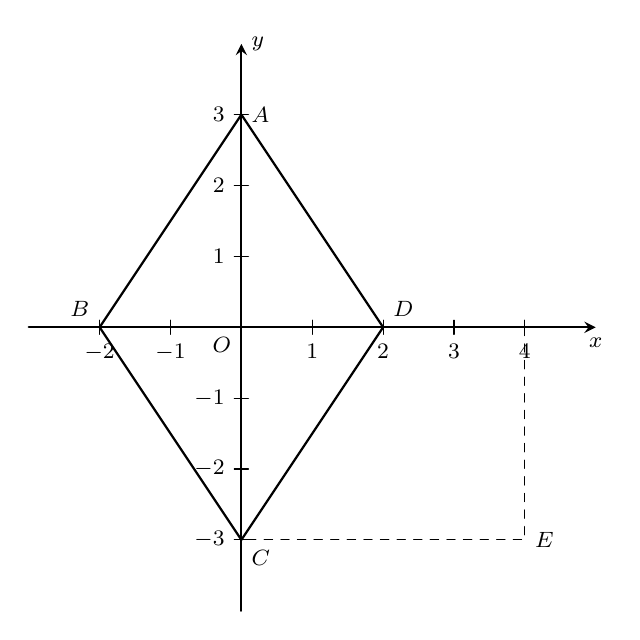
\begin{tikzpicture}[scale=0.9,font=\footnotesize,line join=round,line cap=round,>=stealth]
					\draw[thick] (-2,0)node[above left]{$ B $}--(0,3)node[right]{$ A $}--(2,0)node[above right]{$ D $}--(0,-3)node[below right]{$ C $}--(-2,0) (4,-3)node[right]{$ E $} (0,0)node[below left]{$ O $};
					\draw[dashed] (4,0)--(4,-3)--(0,-3);
					\draw[->,thick] (0,-4)--(0,4)node[right]{$ y $};
					\draw[->,thick] (-3,0)--(5,0)node[below]{$ x $};
					\foreach \x in {-2,-1,1,2,3,4}\draw (\x,0.1)--(\x,-0.1) node [below] { $\x$};
					\foreach \y in {-3,-2,-1,1,2,3}\draw (0.1,\y)--(-0.1,\y) node [left] { $\y$};
				\end{tikzpicture}
			\end{center}
			$\left| z-4+3i \right|=EP$ với $E\left( 4;-3 \right)$ là điểm biều diễn của số phức $z_1=4-3i$.\\
			Từ hình vẽ ta có $m=\min EP=d\left( E,CD \right)$.\\
			Đường thẳng $CD$ có phương trình $3x-2y-6=0$, suy ra $m=\dfrac{12}{\sqrt{13}}$.\\ $\max EP=\max \left\{ EA,EB,EC,ED \right\}$.\\
			Lại có $EA=\sqrt{16+36}=\sqrt{52}$, $EB=\sqrt{9+36}=3\sqrt{5}$, $EC=4$, $ED=\sqrt{9+4}=\sqrt{13}$.\\
			Do đó $M=EA=\sqrt{52}$. Vậy $M\cdot m=24$.
		}
	\end{ex}
\Closesolutionfile{ans}
\subsection{Bảng đáp án}
\inputansbox{8}{ans/ANS-DANG-42}